\documentclass[14pt]{beamer}

\usepackage[brazil]{babel}
\usepackage{fontspec}
%\usepackage{xltxtra}
%\usepackage{xunicode}
\usepackage[UTF8]{ctex}
\usepackage{minted}
\usepackage{qrcode}
\defaultfontfeatures{Mapping=tex-text}

\setbeamercolor{background canvas}{bg=colorlgray}
\setbeamercolor{normal text}{fg=colorhgray}

\usepackage{config/presento}
\input{config/custom-command}

\newcommand*{\affmark}[1][*]{\textsuperscript{#1}}

\begin{document}

\begin{frame}[plain]
  \vfill
  \color{colorblue}\largetext{Urna Eletrônica: Segura?}
  \vfill
  \color{gray}{Relatos do Teste Público de Segurança do Sistema Eletrônico de Votação -- 2017}
  \vfill
  \color{orange}{Caio Lüders, Diego Aranha, Paulo Matias, Pedro Barbosa, Thiago Cardoso}
  \vfill
\end{frame}

\begin{frame}{A Urna Eletrônica Brasileira}
  \begin{fullpageitemize}
  \itemR Projeto de sistema embarcado extremamente complexo
  \itemR Dezenas de milhões de linhas de código
    \begin{itemize}
      \itemR Bootloader customizado pelo TSE
      \itemR Kernel Linux customizado pelo TSE
      \itemR Drivers da Diebold\\(MSD --- \textit{Master Secure Device})
      \itemR Userland do TSE (\texttt{initje})
      \itemR Software da urna em si (\texttt{scue}, \texttt{vota})
    \end{itemize}
  \end{fullpageitemize}
\end{frame}

\begin{frame}{Panorama da área}
  \begin{fullpageitemize}
    \itemR Segurança de software é um\\problema \textbf{difícil}
    \itemR Evolução lenta: ``ainda executamos processos como \textit{root} sob um kernel monolítico escrito em C''
    \itemR 168 CVEs de execução de código arbitrário no kernel Linux só em 2017
  \end{fullpageitemize}
\end{frame}

\begin{frame}{Acidente ou sabotagem?}
  \begin{fullpageitemize}
    \itemR É tão fácil cometer erros de codificação\\que muitas vezes é difícil distinguir\\um erro acidental de uma backdoor
    \vfill
    \includegraphics[width=\textwidth,height=0.45\textheight,keepaspectratio]{images/gotofail_code}
    \vfill
    \includegraphics[width=\textwidth,height=0.45\textheight,keepaspectratio]{images/gotofail}
  \end{fullpageitemize}
\end{frame}

\begin{frame}{Seria a urna imune?}
  \begin{fullpageitemize}
    \itemR A urna \textbf{não} é magicamente imune\\a esses problemas
    \itemR No TPS, nós conseguimos executar\\código arbitrário na urna
    \itemR Corrigir a falha que encontramos\\não garante que não existam outras
  \end{fullpageitemize}
\end{frame}

\begin{frame}{Como tornar a urna segura?}
  \begin{fullpageitemize}
    \itemR Pergunta errada
    \itemR Caminho mais viável:\\ \textit{princípio da independência do software}
    \itemR Linha do tempo
    \begin{itemize}
      \itemR Lei 12.034/09: comprovante impresso
      \itemR Anulado pela ADI 4543 (PGR)
      \itemR Lei 13.165/15: volta do comprovante
    \end{itemize}
  \end{fullpageitemize}
\end{frame}

\begin{frame}{Resistência e preconceito}
  \centering
  \includegraphics[width=\textwidth,height=0.90\textheight,keepaspectratio]{images/tsefaq_votoimpresso}
\end{frame}

\begin{frame}{Nossos objetivos}
  \begin{fullpageitemize}
    \itemR Demonstrar a importância de avançar em direção ao \textit{princípio da independência do software}
    \itemR Inicialmente: explorar o maior número possível de vetores de ataque
    \itemR Devido às dificuldades, mudamos para: explorar \textbf{em profundidade} o primeiro vetor de ataque que encontramos
    \itemR Construir um ataque totalmente\\\textbf{sem premissas}
  \end{fullpageitemize}
\end{frame}

\begin{frame}{Como funcionam os testes?}
  \begin{fullpageitemize}
    \itemR Submetemos \textbf{planos de teste}
    \itemR Os planos de teste são analisados e aprovados pelo TSE
    \itemR Executamos os planos de teste em uma bancada com computador e urna eletrônica
  \end{fullpageitemize}
\end{frame}

\begin{frame}{Planta do ambiente}
  \centering
  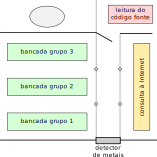
\includegraphics[width=\textwidth,height=0.90\textheight,keepaspectratio]{images/planta}
\end{frame}

\begin{frame}{Dificuldades}
  \begin{fullpageitemize}
    \itemR Entrada de software (em DVD-ROM) ou material impresso apenas após análise e aprovação de \textit{solicitação de material}
    \itemR Regras aplicam-se mesmo para material discriminado nos planos de teste previamente aprovados
    \itemR Proibido transitar com anotações entre ambiente de leitura de código fonte e\\ bancada de testes
    \itemR Problemas para habilitar virtualização nos computadores fornecidos
  \end{fullpageitemize}
\end{frame}

\begin{frame}{Segunda-feira e terça-feira}
  \begin{fullpageitemize}
    \itemR Burocracia
    \itemR Preparação do ambiente
    \vfill
    {\centering
    \includegraphics[width=\textwidth,height=0.90\textheight,keepaspectratio]{images/prep_ambiente}}
  \end{fullpageitemize}
\end{frame}

\begin{frame}{Carga da urna}
  \begin{fullpageitemize}
    \itemR Instalação do SO em uma urna virgem
    \itemR Realizada por meio da inserção de um \textit{cartão de carga}
    \vfill
    {\centering
    \includegraphics[width=\textwidth,height=0.90\textheight,keepaspectratio]{images/criancas_carga}}
  \end{fullpageitemize}
\end{frame}

\begin{frame}{Partições do cartão de carga}
  \begin{fullpageitemize}
    \itemR Partição com o kernel
    \itemR Root do UENUX\\(GNU/Linux embarcado do TSE)
    \itemR Partição com executável do \texttt{vota}
      \begin{itemize}
        \itemR Treinamento
        \itemR Simulação
        \itemR Votação
      \end{itemize}
  \end{fullpageitemize}
\end{frame}

\begin{frame}{Ofuscação}
  \begin{fullpageitemize}
    \itemR Encriptação do kernel
    \itemR Encriptação da partição do UENUX
  \end{fullpageitemize}
\end{frame}

\begin{frame}{Kernel}
  \begin{fullpageitemize}
    \itemR Encriptado com AES'256-ECB
    \itemR Decriptado no boot por \texttt{syslinux} modificado
      \begin{itemize}
        \itemR Acesso ao código fonte completo somente na sexta-feira
      \end{itemize}
    \itemR AES' $\mathbf{\neq}$ AES (!!)
      \begin{itemize}
        \itemR Rounds pares são diferentes\\de rounds ímpares
        \itemR Aparentemente, intercala chaves de rodada de encriptação/decriptação do AES comum
      \end{itemize}
  \end{fullpageitemize}
\end{frame}

\begin{frame}{Partição do UENUX}
  \begin{fullpageitemize}
    \itemR Sistema de arquivos \texttt{ueminix}
      \begin{itemize}
        \itemR Sistema de arquivos \texttt{minix} customizado pelo TSE
        \itemR Estrutura de diretórios e \\nomes de arquivos intactos
        \itemR Conteúdo dos arquivos encriptado individualmente com AES-XTS
      \end{itemize}
  \end{fullpageitemize}
\end{frame}

\begin{frame}{Modo XTS}
  \vfill
  {\centering
  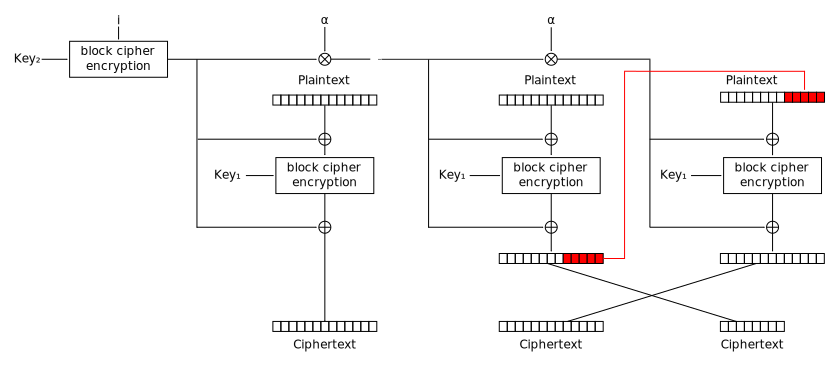
\includegraphics[width=\textwidth,height=0.90\textheight,keepaspectratio]{images/XTS_mode_encryption}}
  \vfill
\end{frame}

\begin{frame}{Encriptação do ueminix}
  \begin{fullpageitemize}
    \itemR IV ($i$): inode do arquivo (consulte com \texttt{ls -i})
    \itemR Chaves:
      \begin{itemize}
        \itemR $\mathrm{Key}_1$: \textit{Hardcoded} no kernel
        \itemR $\mathrm{Key}_2$: Bytes no offset $512+128$ da partição, xor com o byte em $512+7$ (normalmente 0)
      \end{itemize}
    \itemR Modificação com relação ao XTS padrão: reset do $\alpha$ de volta ao IV a cada 4096 bytes
      \begin{itemize}
        \itemR Mais ofuscação
        \itemR Enfraquece (!!) o algoritmo
      \end{itemize}
  \end{fullpageitemize}
\end{frame}

\begin{frame}{Assinaturas (verificação)}
  \vfill
  {\centering
  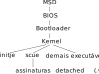
\includegraphics[width=\textwidth,height=0.90\textheight,keepaspectratio]{images/assinaturas_sistema}}
  \vfill
\end{frame}

\begin{frame}{Resumo da quarta-feira}
  \begin{fullpageitemize}
    \itemR Escrevemos um utilitário para ler (decriptando) e escrever (encriptando) partições \texttt{ueminix}
    \itemR Usamos uma chave exfiltrada do código fonte do kernel para o AES-XTS
    \itemR Encontramos bibliotecas compartilhadas que não estavam assinadas $\Rightarrow$ \textbf{vetor de ataque}
  \end{fullpageitemize}
\end{frame}

\begin{frame}{Bibliotecas compartilhadas}
  \begin{fullpageitemize}
    \itemR Execução de código arbitrário no espaço de memória de qualquer processo linkado à biblioteca!
    \itemR Bibliotecas vulneráveis
    \begin{itemize}
      \itemR Log: usada por praticamente todos os executáveis
      \itemR HKDF: usada pelo \texttt{scue} e pelo \texttt{vota}
    \end{itemize}
  \end{fullpageitemize}
\end{frame}

\begin{frame}[fragile]{Ataque simples ao sigilo do voto}
  \begin{fullpageitemize}
    \itemR Substituímos a função \texttt{hkdf} por:
      \begin{minted}{asm}
        xor eax, eax
        ret
      \end{minted}
    \vfill
    \itemR Essa função gera uma chave usada para encriptar o RDV com AES256-CBC
    \itemR Assim, forçamos que o RDV seja encriptado com uma chave zerada
    \itemR RDV só é lido em caso de ``recontagem'': ataque difícil de detectar
  \end{fullpageitemize}
\end{frame}

\begin{frame}{Executando programas na urna}
  \begin{fullpageitemize}
    \itemR Kernel verifica assinatura de executáveis $\Rightarrow$ não podemos trocar \textit{e.g.} o \texttt{initje} por um programa nosso
    \itemR Mas a função de log é chamada\\ pelo \texttt{initje} antes do início da \\interface gráfica
    \itemR Substituímos função de log por código em Assembly de um programa interativo escrito por nós, ou carregamos um ELF estático com \texttt{shellcraft.loader\_append}
  \end{fullpageitemize}
\end{frame}

\begin{frame}{Resumo da quinta-feira}
  \begin{fullpageitemize}
    \itemR Violação do sigilo do voto
    \itemR Violação da integridade do log
    \itemR Execução de código Assembly escrito por nós na urna
    \itemR Tentativa de analisar compactação UPX dos binários da urna $\Rightarrow$ o código que levamos em DVD-ROM estava incompleto!
  \end{fullpageitemize}
\end{frame}

\begin{frame}{Modificando o software de votação}
  \begin{fullpageitemize}
    \itemR Escrever um exploit sem ter um depurador
      \begin{itemize}
        \itemR Necessário análise estática
        \itemR Necessário descompactar o UPX
      \end{itemize}
    \itemR Ausência de PIE (\textit{position independent executable}) na urna
      \begin{itemize}
        \itemR Incompatível com UPX?
        \itemR Impede randomização de endereços do executável principal
        \itemR Endereços fixos facilitam a \\escrita do exploit
      \end{itemize}
  \end{fullpageitemize}
\end{frame}

\begin{frame}[fragile]{Em qual executável estamos?}
  \begin{fullpageitemize}
    \itemR Gostaríamos de modificar somente o \texttt{vota}
    \itemR Procuramos um endereço que exista tanto no \texttt{vota} quanto no \texttt{scue}, mas com conteúdo diferente
    \begin{minted}{asm}
mov eax, endereco
mov eax, [eax]
cmp eax, conteudo_esperado
jne nao_eh_o_vota
; altera memória
nao_eh_o_vota:
    \end{minted}
  \end{fullpageitemize}
\end{frame}

\begin{frame}{Mudança de strings}
  \begin{fullpageitemize}
    \itemR Strings constantes ficam na seção \texttt{.rodata}
    \itemR Mudamos permissão de páginas de memória somente-leitura (syscall \texttt{mprotect})
    \itemR Sobrescrevemos endereços conhecidos (\texttt{stosd/w/b})
  \end{fullpageitemize}
\end{frame}

\begin{frame}{Urna que faz boca de urna}
  \vfill
  {\centering
  \includegraphics[width=\textwidth,height=0.90\textheight,keepaspectratio]{images/vote99}}
  \vfill
\end{frame}

\begin{frame}{Infecção furtiva da urna}
  \begin{fullpageitemize}
    \itemR Técnica de \textit{infecção de ELF}\\ na biblioteca HKDF
    \itemR Desviamos o fluxo da função original para área inútil da biblioteca (ou usamos LIEF)
    \itemR Adicionamos código novo mantendo a funcionalidade do original
  \end{fullpageitemize}
\end{frame}

\begin{frame}{Alteração do voto}
  \begin{fullpageitemize}
    \itemR Alterar somente o voto registrado pela urna
    \itemR Não alterar o voto observado\\ pelo eleitor na tela
  \end{fullpageitemize}
\end{frame}

\begin{frame}[fragile]{Método que registra o voto}
  \begin{minted}{c++}
void InfoEleitor::AdicionaVoto(
    uint8_t cargo,
    int tipo,
    std::string &voto)
{
    cedula->AdicionaVoto(Voto(cargo,
                              tipo,
                              voto));
    LogaVoto(cargo, tipo);
}
  \end{minted}
\end{frame}

\begin{frame}[fragile]{Validação de hipótese}
  \begin{fullpageitemize}
    \itemR Substituímos o método \texttt{AdicionaVoto} por:
      \begin{minted}{asm}
        ret
      \end{minted}
    \vfill
    \itemR Eleitor entra com votos para todos os cargos
    \itemR Logo antes da tela de FIM, aparece a mensagem de erro: ``cédula vazia''
  \end{fullpageitemize}
\end{frame}

\begin{frame}{Resumo da sexta-feira}
  \begin{fullpageitemize}
    \itemR Visita do ministro
    \itemR Descompactação do UPX
    \itemR Violação da integridade do\\ software de votação
    \itemR Exploits para troca de strings e alteração de cédulas de votação
    \itemR Quebra do bootloader pela equipe do Peixinho, complementando nosso ataque e tornando-o completamente sem premissas
  \end{fullpageitemize}
\end{frame}

\begin{frame}[fragile]{O que faríamos com mais tempo?}
  \begin{fullpageitemize}
    \itemR Testar o exploit de alteração de voto na urna
    \begin{itemize}
      \itemR Testamos código infectado do método \texttt{AdicionaVoto} no PC: funcionou
      \itemR Mas cada carga demora $\approx$~30~min
    \end{itemize}
    \itemR Burlar votação paralela
    \begin{itemize}
      \itemR Código para \texttt{AdicionaVoto} ligeiramente mais complexo
      \begin{minted}{c++}
if (voto == "99123") {
  ativa_mutreta();
}
      \end{minted}
    \end{itemize}
  \end{fullpageitemize}
\end{frame}

\begin{frame}{Conclusão}
  \begin{fullpageitemize}
    \itemR Explorar a urna é conceitualmente o mesmo que fazer \textit{jailbreak} em iPhone
    \itemR Falhas acontecem
    \itemR O \textit{princípio da independência do software} é importante!
  \end{fullpageitemize}
\end{frame}

%\begin{frame}{Acesse}
%  \begin{center}
%  \qrcode[height=4cm]{https://github.com/org/proj}\\[1em]\small\url{https://github.com/org/proj}
%  \end{center}
%\end{frame}

\end{document}
